\chapter{Fashion Survey}
\label{chap:survey}

Fashion bloggers and social media in a more general way are becoming an influential force within the fashion industry. Fashion related applications pulls data from Instagram and other social media platform in order to enlarge their datasets and consolidate it. The purpose of this survey is to extract more features and discover platforms that are used to spot new clothing trend. In a first part, we present the survey and in the second part, we describe the survey’s analysis and results.

%%%%%%%%%%%%%%%%%%%%%%%%%%%%%%%%%%%%%%%%%%%%%%%%%%%%%%%%%%%%%%%%%%%%%%%%%%%%%%%%%%%%%%%%%%%%%%%%%%
%%%%%%%%%%%%%%%%%%%%%%%%%%%%%%%%%%%%%%%%%%%%%%%%%%%%%%%%%%%%%%%%%%%%%%%%%%%%%%%%%%%%%%%%%%%%%%%%%%
\section{Presentation}
This survey was performed on \ac{CF} asking 800 men and women from 16 European countries questions about their online shopping habits. The choice of the 16 European countries was based on Zalando’s delivery destinations. When the participants accepts the task (or accesses the system web page), they will be asked to read the Information Sheet and Consent Form and indicate their agreement and this is the first page of the system. Then, the participants are given an entry questionnaire to gather demographic information such as age, gender, nationality, etc. Next, each participant will be presented with a series of questions about his/her social media habits, his/her behaviour towards fashion blogs and preferred content presentation in both retailer websites and social media platforms. The results of the survey are described in the following section.

%%%%%%%%%%%%%%%%%%%%%%%%%%%%%%%%%%%%%%%%%%%%%%%%%%%%%%%%%%%%%%%%%%%%%%%%%%%%%%%%%%%%%%%%%%%%%%%%%%
%%%%%%%%%%%%%%%%%%%%%%%%%%%%%%%%%%%%%%%%%%%%%%%%%%%%%%%%%%%%%%%%%%%%%%%%%%%%%%%%%%%%%%%%%%%%%%%%%%
\section{Results and Analysis}
\subsection{Shopping Online/ Social Media Habits}

Online shopping is becoming increasingly popular for multiple reasons. People find it more convenient because it saves time, it is available 24/7 and the comparison between products can be made in few clicks.  Clothes shopping is not an exception, among the 800 men and women we asked, 94.7\% of them shopped clothes online at least once. These digital buyers turn to social media for a variety of reasons like reading comments and discovering new trends. For instance, 75\% of the participants who check their social media account several times a day, use them to follow fashion trend.
While a clear majority use social media to follow new clothing trends, the platform choice differs slightly depending on the age and the gender. Figure~\ref{fig:gender_pref} shows the top platforms depending on the gender. We can see that \ac{FB} is the most popular platform for both men and women, Instagram and \ac{YT} are ranked just behind, then Pinterest who is more popular among women more than men. 

\begin{figure}[htb] \centering 
  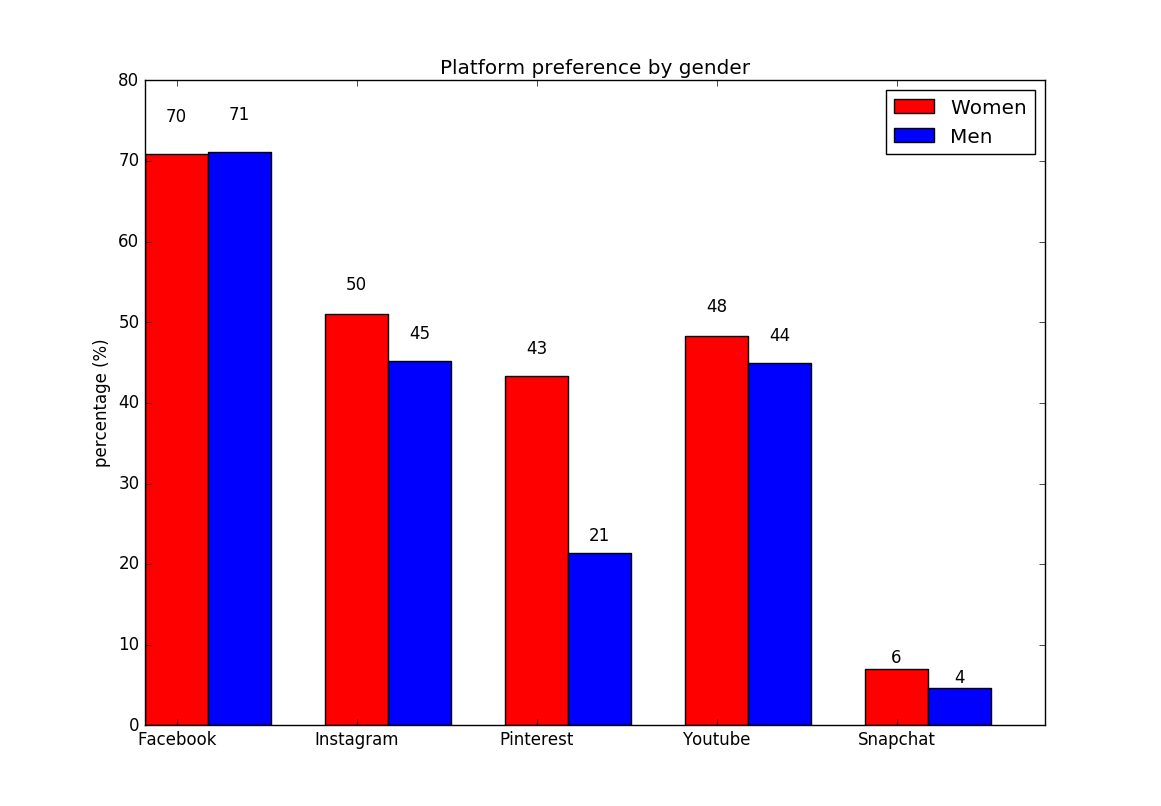
\includegraphics[scale=0.4]{gender_pref}
  \caption{Platform preference by gender.}
  \label{fig:gender_pref}
\end{figure}


The preference for the social media platform depending on the age range is shown in Figure~\ref{fig:age_pref}. \ac{FB} has a uniform and large user base (2 billion monthly active users in 2017) which explains why 70\% of each age range chooses \ac{FB} to discover Fashion trend. Instagram is the second choice with more popularity among the younger generation (under 30). Around half of each age range uses \ac{YT}, then we have Pinterest and Snapchat ranked just behind.


\begin{figure}[htb] \centering 
  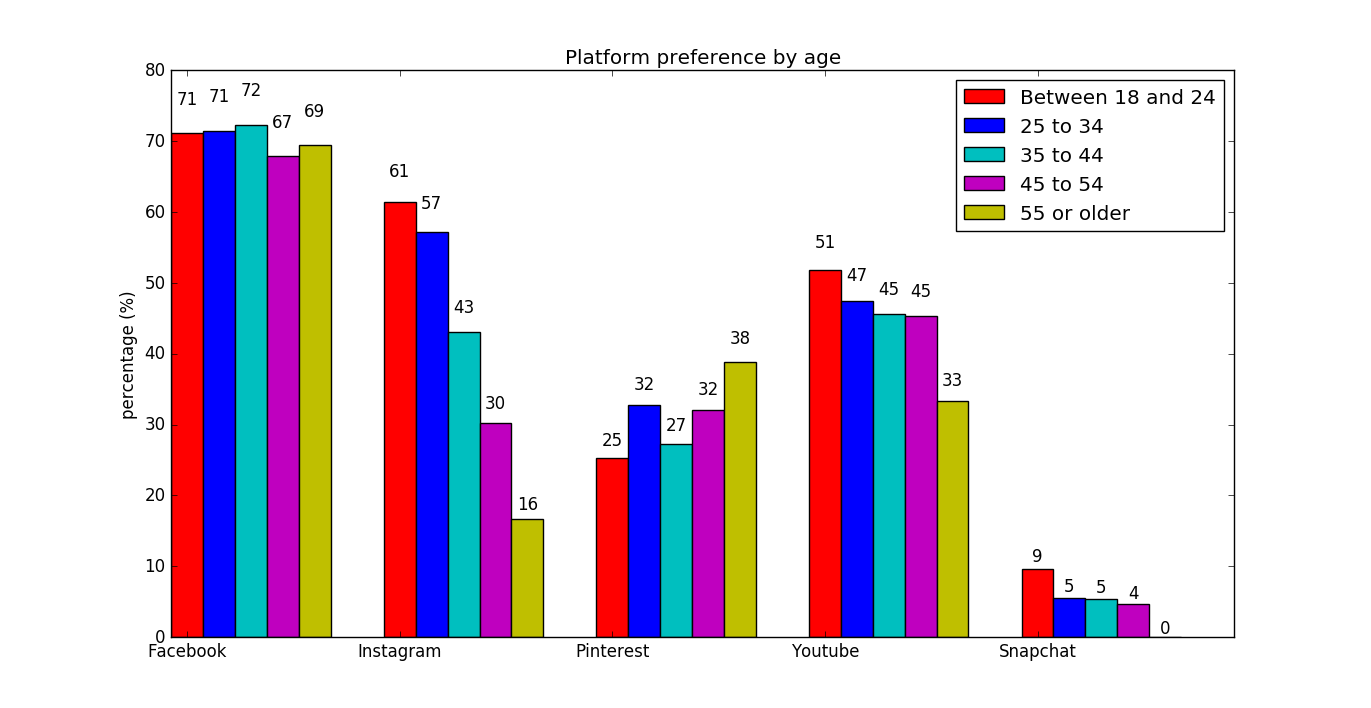
\includegraphics[scale=0.4]{age_pref}
  \caption{ Platform preference for discovering clothing trend by age.}
  \label{fig:age_pref}
\end{figure}



The results of the survey show that the majority of the participants, i.e., 71.8\% of them, uses \ac{FB} platform to discover new fashion trends. When studying the demographic of this majority, around 70\% of each age range uses this platform to discover new trends. This result was expected since the user base of \ac{FB} is uniform. Besides reaching a large community, a \ac{FB} post has more opportunity for getting feedback of all kinds and is more likely to get a deeper level of interaction since the comments can contain text, emoji and images unlike other platforms where only text/emoji are allowed. 

According to the survey results, Instagram is the second platform to be used in order to spot new clothing trends, i.e. 49.1\% of the participants. A majority of these Instagram users are under 30 as a matter of fact, this platform appeals more to the younger generation at the opposite of Pinterest that is slightly more popular in older generations. Almost half of the participants use \ac{YT} to discover fashion. As a matter of fact, in June 2016, beauty-related content generated more than 5 billion views per month. Popular types of \ac{YT} beauty content include tutorials, reviews, and videos produced by beauty vloggers~\cite{stat}.

Since \ac{FB} and Instagram are the most popular platforms to discover fashion according to the survey results, we will briefly describe the difference between the two platforms. \ac{FB} is focused more on text and is largely informational while, Instagram is more about “capturing the moment”. It is also worth mentioning that \ac{FB} content is so diverse that one can easily get distracted, while Instagram focuses on image/video sharing only. Users are more able to be engaged with the visual content shared on Instagram which explains why when asking participants to name fashion influencers they know, we count only 9 \ac{FB} pages while  87 fashion instagram accounts. The difference between the number of \ac{FB} pages and the number of instagram accounts mentioned bring us to conclude that while \ac{FB} has the largest user base, Instagram audience is more engaged. This last result suggests that social media platforms have a key role in creating, advertising and spreading clothing trends. Hence, social media data will play a pivotal role in the rest of our project. Since social media data often comes in an unstructured format, the ensuing data integration task will consist of recognizing key entities to be linked with our fashion catalog (Fashion Knowledge Base), this will be done either via text or image processing.

This question revealed some other platforms used to discover fashion trend like Reddit 21 buttons, google+, Soup.io, lookbook, bantoa, elcorteingles, etc.

\subsection{Influence of Bloggers and Social Media on Their Viewers}

In this section, we gather the results related to how participants use social media to discover fashion trends and who are the influencers they follow to spot new trends.
A common way to stay updated with the latest trend is to follow brands on social media. For instance, 63.6\% of the participants follow their favourite brands on social media. They also find the best way to get inspiration about what clothing to purchase is going through online clothing shops (75.5\%) and by following them on social media (48.6\%). These methods beat by far the traditional way of looking into magazines (27.5\%) and visual merchandising in shops (34.2\%). Therefore, social media platforms are not only used to discover trend but also have an influence on people's decision to purchase items. As shown in the chart of Figure~\ref{fig:freq}, 44.8\% of the participants frequently purchase items discovered through social media. 


\begin{figure}[htb] \centering 
  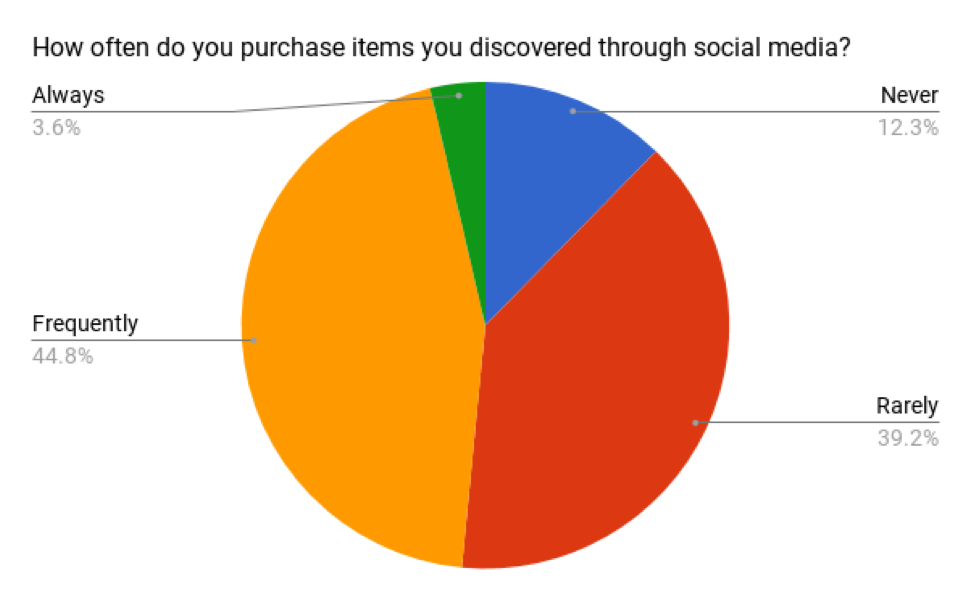
\includegraphics[scale=0.5]{influence_bloggers}
  \caption{Frequency of purchased items discovered through Social Media.}
  \label{fig:freq}
\end{figure}

Below some answers to the question “Describe how you use social media to discover fashion trends”:
“I visit profiles of people who publish photos and reviews of clothes from new collections of well-known brands. I also visit the profiles with ideas how to join various pieces of clothing to make a great and fashionable outlook.”
“\ac{FB} and Twitter are great for discovering new trends, and Pinterest is wonderful for a visual experience.”
These answers reveal how fashion bloggers are gaining a lot of popularity and have a clear influence on their followers as a matter of fact 40\% of the participants use fashion blogs to have an idea about their next shopping.
The participants provided us with 168 distinct blogs, \ac{YT} channels and Instagram accounts (The list is kept in our shared repository). We name here those with the highest number of followers:

\begin{itemize}
    \item @chiaraferragni
    \item @songofstyle 
    \item @galagonzalez
    \item @thefashionguitar
\end{itemize}

From this list we can hypothesis that the list of influencers is large and growing which makes it difficult to keep up manually. The recommendation that we issue for (WP3) is the development of an interface for the continuous collection and curation of an influencer list by means of crowdsourcing.


\subsection{Comments/Reviews}


Users share their feelings and opinions on products mostly to clarify some doubts before purchasing (48.8\%) or to give some subjective feedback afterwards (41\%) as depicted in Figure~\ref{fig:perc}. The most important aspects participants look for in a review are: (i) the item’s general features specially the quality of the product and (ii) whether is it similar to the picture and description.


\begin{figure}[htb] \centering 
  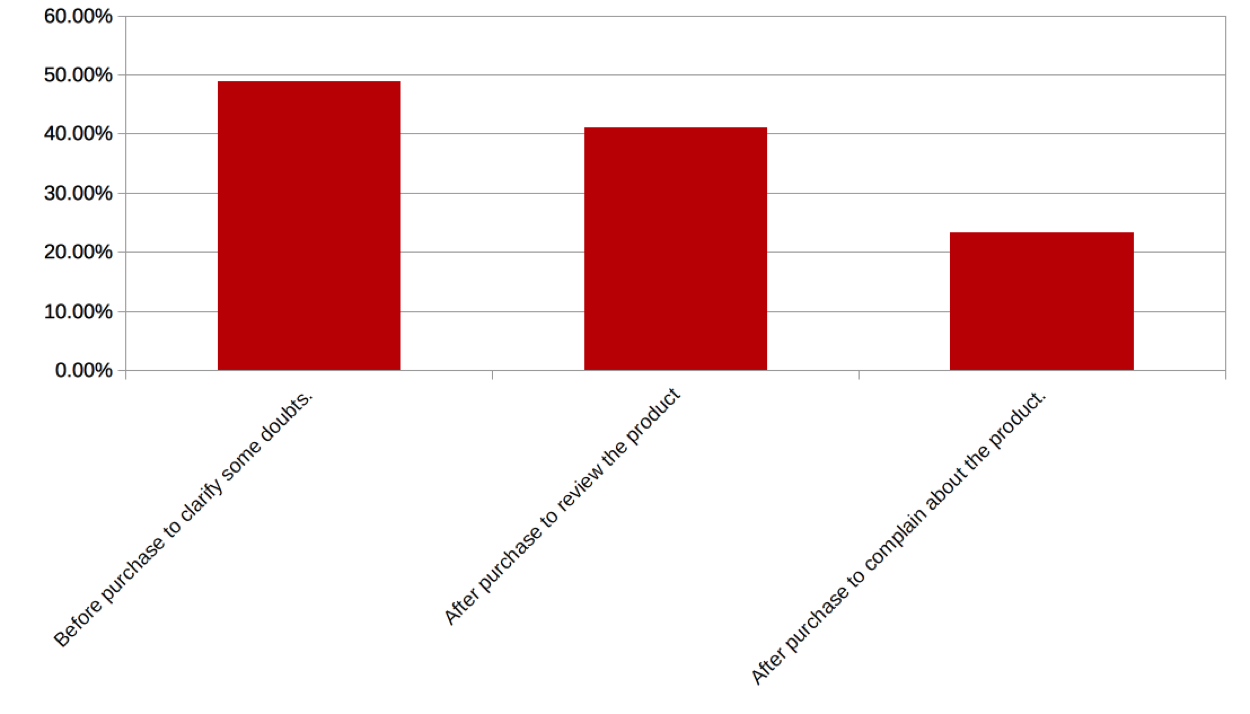
\includegraphics[scale=0.6]{images/figs/comments_reviews}
  \caption{Percentage of participants answering: When are you more likely to review or comment about a fashion product?}
  \label{fig:perc}
\end{figure}


With social media, regular consumers have a direct access to fashion designers, clothing and shoes firms. When fashion companies do social media marketing, they are more able to reach and engage a wider audience. When asking the participants “how do you interact with fashion brands on social media?”, we found as depicted in Figure~\ref{fig:inter} , 43\% of them answering by “liking posts/publications” and 25\% of them by “commenting on posts/publications”. Therefore, it is possible to measure the popularity of a specific trend or style with the number of likes and comments. This same approach was used in different domain such as prediction of the new popular models~\cite{Park:2016:SAI:2818048.2820065} and the box-office performance of newly-released blockbuster movies~\cite{Asur11}.


\begin{figure}[htb] \centering 
  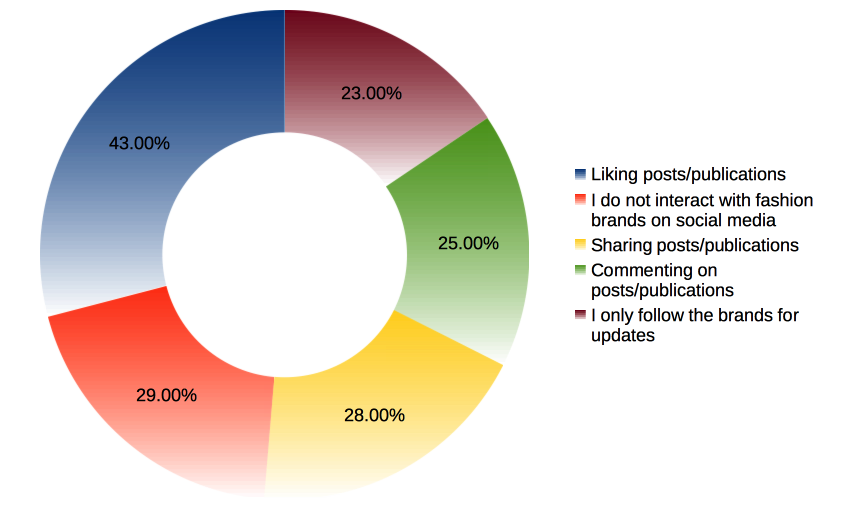
\includegraphics[scale=0.6]{interaction}
  \caption{Interaction with fashion brands.}
  \label{fig:inter}
\end{figure}

\subsection{Fashion Content}

In this section, we describe the preference of data type according to the survey participants  (image, text, videos) and how they prefer items to be displayed.
  
Figure~\ref{fig:content} shows that image is the preferred content users want to see on fashion social media then comes videos and text consecutively. Even though videos seem to have less importance compared to image, they are an important source of information to spot new trends. For example, the participants provided us with around 30 distinct \ac{YT} channels dedicated to fashion. Such a high number of fashion videos shows that the latter are fashion drivers.


\begin{figure}[htb] \centering 
  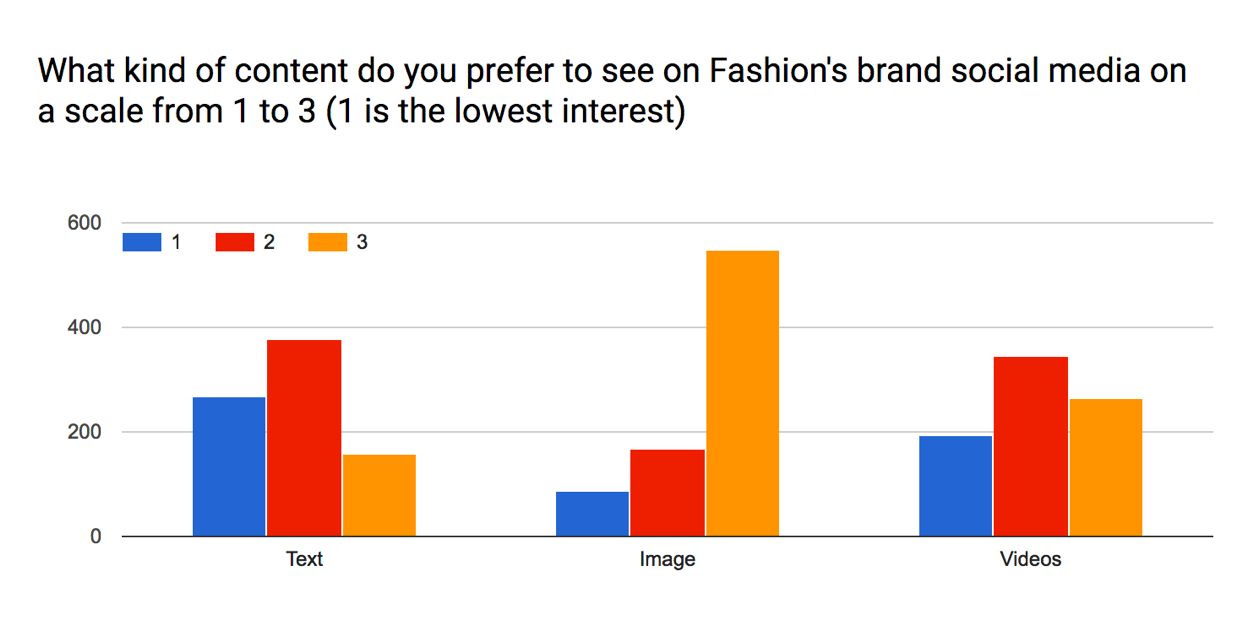
\includegraphics[scale=0.6]{content_pref}
  \caption{Content type preference.}
  \label{fig:content}
\end{figure}



Items on models and showing a combination of items is preferred over focusing on showing items solely as shown in Figure~\ref{fig:focus}. Thus, for the image processing tasks, we recommend to take into account overall style recommendation, i.e., combination of multiple items instead of focusing on showing different items separately.


\begin{figure}[htb] \centering 
  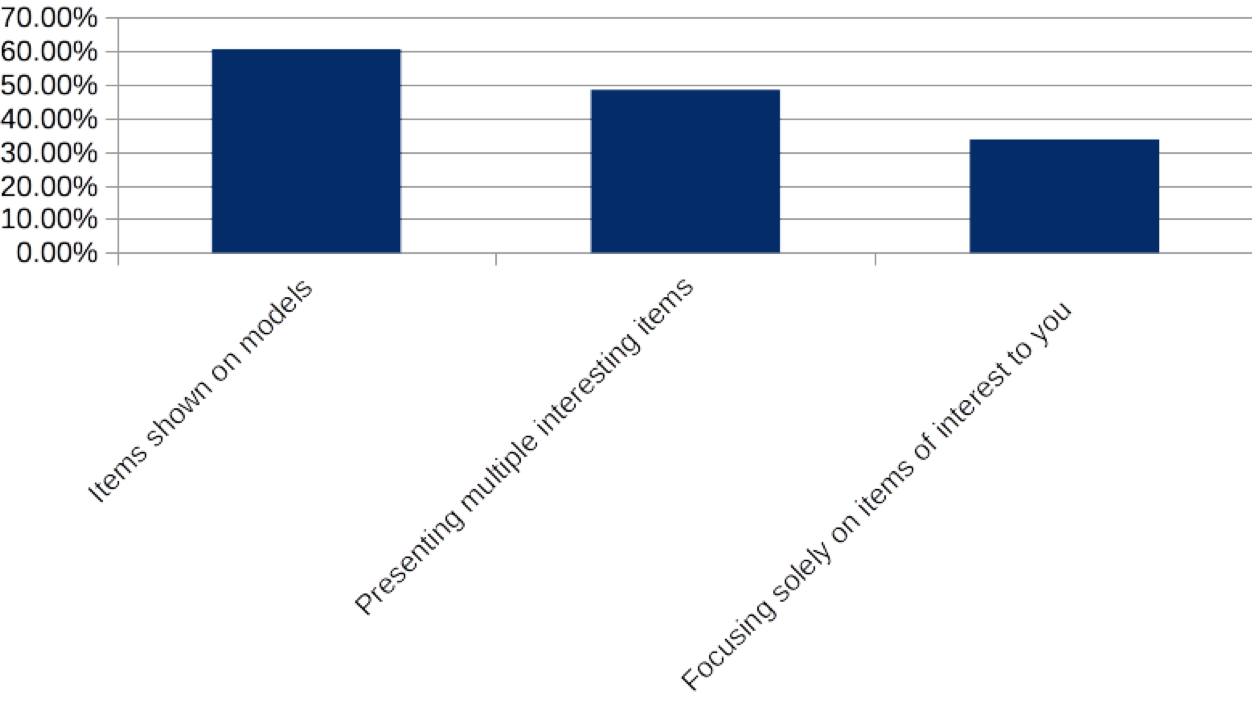
\includegraphics[scale=0.6]{focus_pref}
  \caption{Focus preference.}
  \label{fig:focus}
\end{figure}

\subsection{Other Forms of Content}


VR and AR are still in early development stages. However as technology becomes mainstream, with companies like \ac{FB} and Snapchat investing millions in R\&D, these technologies are expected to be integrated in the social media experience quite soon. Fashion related applications are already launched and even though they were not mentioned by the 800 participants, they will soon become a powerful channel for brand-consumer interaction : 

\begin{itemize}
    \item Uniqlo’s Magic Mirror: Uniqlo offered shoppers the unique ability to imagine themselves in a range of color choices of a single silhouette without the hassle of having to remove the garment.
    \item The Sampler mobile app from Converse: A mobile application that gives people the ability to imagine what a Converse product would look like on-foot without having to actually try on a pair. One has only to point his iPhone camera at his leg and subsequently getting a visual reference on how it would look.
\end{itemize}

We add as a target in WP3 the tracking of the adoption of new technologies.